\documentclass[10pt, landscape]{article}
\usepackage[scaled=0.92]{helvet}
\usepackage{calc}
\usepackage{multicol}
\usepackage[a4paper,margin=3mm,landscape]{geometry}
\usepackage{amsmath,amsthm,amsfonts,amssymb}
\usepackage{dsfont}
\usepackage{color,graphicx,overpic}
\usepackage{hyperref}
\usepackage{newtxtext} 
\usepackage{enumitem}
\usepackage[table]{xcolor}
\usepackage{mathtools}
\setlist{nosep}
% for including images
\graphicspath{ {./images/} }

\pdfinfo{
  /Title (CS3236.pdf)
  /Creator (TeX)
  /Producer (pdfTeX 1.40.0)
  /Author (Jovyn Tan)
  /Subject (CS3236)
/Keywords (CS3236, nus,cheatsheet,pdf)}

% Turn off header and footer
\pagestyle{empty}

% redefine section commands to use less space
\makeatletter
\renewcommand{\section}{\@startsection{section}{1}{0mm}%
  {-1ex plus -.5ex minus -.2ex}%
  {0.5ex plus .2ex}%x
{\normalfont\large\bfseries}}
\renewcommand{\subsection}{\@startsection{subsection}{2}{0mm}%
  {-1explus -.5ex minus -.2ex}%
  {0.5ex plus .2ex}%
{\normalfont\normalsize\bfseries}}
\renewcommand{\subsubsection}{\@startsection{subsubsection}{3}{0mm}%
  {-1ex plus -.5ex minus -.2ex}%
  {1ex plus .2ex}%
{\normalfont\small\bfseries}}%
\makeatother

\renewcommand{\familydefault}{\sfdefault}
\renewcommand\rmdefault{\sfdefault}
%  makes nested numbering (e.g. 1.1.1, 1.1.2, etc)
\renewcommand{\labelenumii}{\theenumii}
\renewcommand{\theenumii}{\theenumi.\arabic{enumii}.}
\renewcommand\labelitemii{•}
\renewcommand\labelitemiii{•}

\definecolor{mathblue}{cmyk}{1,.72,0,.38}
\everymath\expandafter{\the\everymath \color{mathblue}}

% Don't print section numbers
\setcounter{secnumdepth}{0}

\setlength{\parindent}{0pt}
\setlength{\parskip}{0pt plus 0.5ex}
%% adjust spacing for all itemize/enumerate
\setlength{\leftmargini}{0.5cm}
\setlength{\leftmarginii}{0.5cm}
\setlist[itemize,1]{leftmargin=2mm,labelindent=1mm,labelsep=1mm}
\setlist[itemize,2]{leftmargin=4mm,labelindent=1mm,labelsep=1mm}

% adding my commands
% tightcenter
\newenvironment{tightcenter}{%
  \setlength\topsep{0pt}
  \setlength\parskip{0pt}
  \begin{center}
    }{%
  \end{center}
}

% boxed
\newenvironment{tightbox}{%
  \setlength\topsep{0pt}
  \setlength\parskip{0pt}
  \begin{center}
    \begin{tabular}{|@{\hspace{\dimexpr\fboxsep+0.5\arrayrulewidth}}c@{\hspace{\dimexpr\fboxsep+0.5\arrayrulewidth}}|}
      \hline
    }
    {%
    \\ \hline
    \end{tabular}
  \end{center}
}

% fixed width box
\newenvironment{fixedbox}[1][0.7]{
  \setlength\topsep{0pt}
  \setlength\parskip{0pt}
  \begin{center}
    \begin{tabular}{|>{\centering\arraybackslash}m{#1\linewidth}|}
    \hline
  }{
  \\ \hline
  \end{tabular}
  \end{center}
}

% definition of a new term
\usepackage{soul}
\definecolor{paleyellow}{RGB}{251,243,218}
\newcommand{\definition}[2][]{\sethlcolor{paleyellow}\hl{\textbf{#2}} #1  $\rightarrow$}

% important note (attention)
\newcommand{\attention}{{\color{red}\textbf{! }}}


%  convenient absolute value symbol
\newcommand{\abs}[1]{\vert #1 \vert}

%  convenient floor and ceiling
\newcommand{\floor}[1]{\lfloor #1 \rfloor}
\newcommand{\ceil}[1]{\lceil #1 \rceil}

%  modulo with nicer spacing
\newcommand{\Mod}[1]{\ \mathrm{mod}\ #1}

%  convenient dx with nicer spacing
\newcommand{\dx}{\mathop{dx}}


\DeclareMathOperator*{\argmax}{arg\,max}
\DeclareMathOperator*{\argmin}{arg\,min}

% -----------------------------------------------------------------------

\begin{document}
\raggedright
\footnotesize
\begin{multicols*}{4}
  % multicol parameters
  \setlength{\columnseprule}{0.25pt}

  \begin{center}
    \fbox{%
      \parbox{0.8\linewidth}{\centering \textcolor{black}{
          {\Large\textbf{CS3236}}
        \\ \normalsize{AY22/23 SEM 2}}
        \\ {\footnotesize \textcolor{gray}{github/jovyntls}}
      }%
    }
  \end{center}

  \section{01. INFORMATION MEASURES}

  $X$ is a d.r.v. with pmf $P_X$ over an alphabet $\mathcal{X}$ (set of symbols)
  \begin{itemize}
    \item speed: \definition{rate} $\frac{k}{n}$ (mapping $k$ bits to $n$ bits)
  \end{itemize}

  \subsection{information of an event: $\psi(\cdot)$}


  \begin{minipage}[c]{0.23\linewidth}
    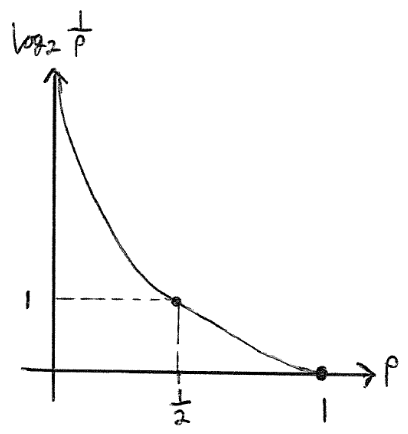
\includegraphics[width=\linewidth]{cs3236-information-log2-p-graph.png} 
  \end{minipage}
  \begin{minipage}[c]{0.74\linewidth}\color{black}
    \begin{tightcenter}
      $ \psi(p) = \log_b \frac{1}{p} $ (for some $b>0$)
    \end{tightcenter}
    \begin{itemize}
      \item all choices of $b$ are equivalent up to scaling by a universal constant
        \begin{itemize}
          \item e.g. \# of nats $= \log_e 2 \times$ \# of bits
        \end{itemize}
    \end{itemize}
  \end{minipage}

  \begin{enumerate}
    \item $\psi(p) \geq 0\quad$ (\textbf{non-negativity}) 
    \item $\psi(1) = 0\quad$ (\textbf{zero for definite events}) 
    \item if $p \leq p'$, then $\psi(p) \geq \psi(p') \quad$ (\textbf{monotonicity})
    \item $\psi(p)$ in continuous in $p \quad$ (\textbf{continuity}) 
    \item $\psi(p_1 p_2) = \psi(p_1) + \psi(p_2)$
      (\textbf{additivity under indep})
  \end{enumerate}

  \begin{tightcenter}
    if $X$ takes $N$ values with $\mathbf{p} = (p_1, \dots, p_N)$,

    only  $\Phi(\mathbf{p}) = constant \times H(X)$ satisfies
  \end{tightcenter}

  \begin{enumerate}
    \item if $p_i= \frac{1}{N}$, then $\Psi(\mathbf{p}) $ is increasing in $N$ (\textbf{uniform case})
    \item (\textbf{successive decisions}) $\Psi(p_1, \dots, p_N) = \Psi(p_1 + p_2, p_3, \dots, p_N) + (p_1 + p_2) \Psi (\frac{p_1}{p_1 + p_2}, \frac{p_2}{p_1 + p_2})$
  \end{enumerate}


  \subsection{information of a random variable: $H(X)$}

  \begin{tightcenter}
    \definition{(Shannon) entropy} average information/uncertainty
    \begin{align*}
      H(X) &= \mathbb{E }_{X \sim P_X} \left[ \log_2 \frac{1}{P_X(X)} \right] 
        \\ &= \sum_x P_X(x) \log_2 \frac{1}{P_X(x)}
    \end{align*}
  \end{tightcenter}

  \begin{minipage}[c]{0.77\linewidth}
    \color{black}
    \begin{tightcenter}
      \ildefinition{binary entropy function} 

      $ H_2(p) = p\log_2 \frac{1}{p} + (1-p) \log_2 \frac{1}{1-p} $
    \end{tightcenter}
    \begin{itemize}
      \item binary source: $X \sim Bernoulli(p)$ \\* $\quad \Rightarrow H(X) = H_2(p)$
    \end{itemize}
  \end{minipage}
  \begin{minipage}[c]{0.2\linewidth}
    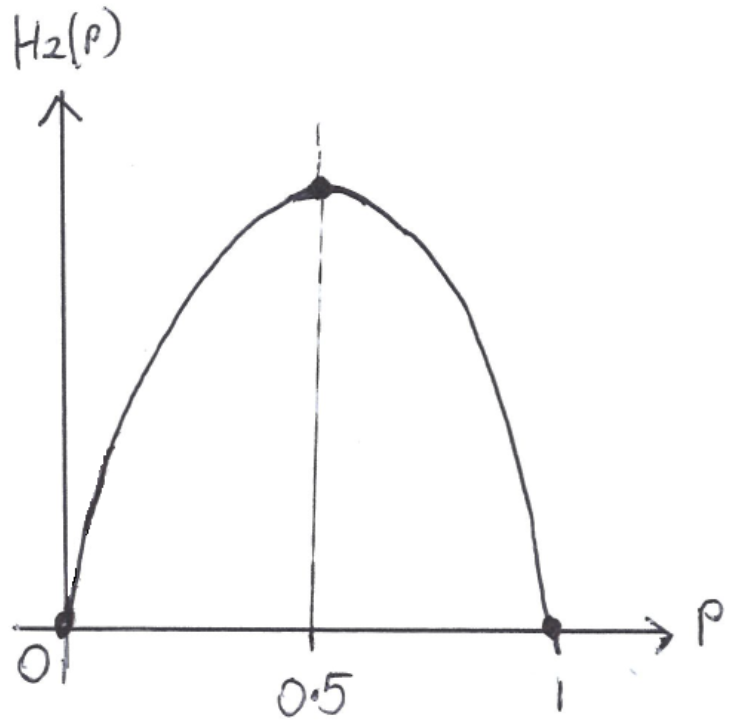
\includegraphics[width=\linewidth]{cs3236-binary-entropy-fn.png} 
  \end{minipage}

  \begin{itemize}
    \item uniform source ($\scriptscriptstyle P_X(x) = \frac{1}{\vert \mathcal{X} \vert}$): \\*
      $\quad \Rightarrow$ $H(X) = \mathbb{E} \left[ \log_2 \frac{1}{1/\vert\mathcal{X}\vert} \right] = \log_2 \vert\mathcal{X}\vert$
  \end{itemize}

  \subsubsection{variations}

  \begin{itemize}
    \item \definition[ of two random variables $(X, Y)$ ]{joint entropy}
      \begin{align*}
        H(X,Y) &= \mathbb{E}_{(X, Y)\sim P_{XY}} \left[ \log_2 \frac{1}{P_{XY}(X,Y)} \right] 
            \\ &= \sum_{x,y} P_{XY} (x,y) \log_2 \frac{1}{P_{XY}(x,y)}
      \end{align*}
    \item \definition[ of $Y$ given $X$ ]{conditional entropy}
      \begin{align*}
        H(Y\vert X) &= \mathbb{E}_{(X,Y) \sim P_{XY}} \left[ \log_2 \frac{1}{P_{Y\vert X}(Y\vert X)} \right] 
                 \\ &= \sum_{x, y} P_{XY}(x,y) \log_2  \frac{1}{P_{Y\vert X}(y\vert x)}
                 \\ &= \sum_x P_X(x) H(Y \vert X=x)
      \end{align*}
      \begin{itemize}
        \item on average, $H(Y\vert X) \leq H(Y)$
          but a \textit{specific} outcome of $X$ may increase uncertainty ($H(Y \vert X=i) > H(Y)$)
      \end{itemize}
  \end{itemize}

  \subsection{properties of entropy}

  \begin{enumerate}
    \item $H(X) \geq 0 \quad$ (\textbf{non-negativity}) equality  $\Leftrightarrow$ deterministic
    \item $H(X) \leq \log_2 \vert\mathcal{X}\vert \quad$ (\textbf{upper bound}) 
      \begin{itemize}
        \item equality $\iff X\sim Uniform(\mathcal{X})$
      \end{itemize}
    \item $H(X, Y) = H(X) + H(Y\vert X) \quad$ (\textbf{chain rule})
      \\* $H(X, Y) = H(Y) + H(X\vert Y)$
      \begin{itemize}
        \item conditioning: $H(X, Y \vert Z) = H(X \vert Z) + H(Y \vert X, Z)$
        \item general chain rule: $H(X_1, \dots, X_n) = \sum^n_{i=1} H(X_i \vert X_1, \dots, X_{i-1})$
      \end{itemize}
    \item $H(X \vert Y) \leq H(X) \quad$ (\textbf{conditioning reduces entropy})
      \begin{itemize}
        \item equality $\iff X$ and $Y$ are independent
      \end{itemize}
    \item $H(X_1, \dots, X_n) \leq \sum^n_{i=1} H(X_i) \quad$ (\textbf{sub-additivity})
      \begin{itemize}
        \item equality $\iff X$ and $Y$ are independent
      \end{itemize}
  \end{enumerate}

  \subsection{KL Divergence}

  \begin{tightcenter}
    \ildefinition{Kullback-Leibler (KL) divergence} or \ildefinition{relative entropy} is
    \begin{align*}
      D(P||Q) &= \sum_x P(x) \log_2 \frac{P(x)}{Q(x)} \\*
              &= \mathbb{E}_{X \sim P}  \left[ \log_2 \frac{P(X)}{Q(X)} \right]
    \end{align*}
  \end{tightcenter}

  \begin{itemize}
    \item $D(P||Q) \neq D(Q||P)$
    \item $D(P||Q) \geq 0, \quad$ equality $\iff P=Q$
      \begin{itemize}
        \item \textit{Proof.} $-D(P||Q) = - \sum_x P(x) \log_2 \frac{P(x)}{Q(x)}$  
          $\leq \sum_x P(x) (\frac{Q(x)}{P(x)}-1) = \sum_x Q(x) - \sum_x P(x) = 0$ 
          \\* (using property that $\log \alpha \leq \alpha-1$, equality iff $\alpha=1$)
      \end{itemize}
    \item $D(P_{XY}\vert\vert P_X P_Y)$ = how far $X,Y$ are from independent
  \end{itemize}

  \subsection{Mutual Information}
  \begin{align*}
    I(X;Y) &= H(Y) - H(Y \vert X) \\*
           &= H(X) - H(X \vert Y) \\*
           &= H(X) + H(Y) - H(X, Y) \\*
           &= D(P_{XY}\vert\vert P_X \times P_Y)
  \end{align*}

  \begin{itemize}
    \item \definition[, $I(X;Y)$]{mutual information} the amount of information we learn about $Y$ by observing $X$ (on avg)
    \item \definition{joint mutual information} 
      \begin{align*}
        I(X_1, X_2 ; Y_1, Y_2) = H(Y_1, Y_2) - H(Y_1, Y_2 \vert X_1, X_2)
      \end{align*}
    \item \definition{conditional mutual information} 
      \begin{align*}
        I(X;Y \vert Z) = H(Y \vert Z) - H(Y \vert X,Z)
      \end{align*}
    \item if  $X=Y$, then $I(X;Y) = H(X) = H(Y)$
  \end{itemize}

  \subsubsection{properties of mutual information}

  \begin{enumerate}
    \item $I(X; Y) = I(Y;X) \quad$ (\textbf{symmetry})
    \item $I(X;Y) \geq 0 \quad $ (\textbf{non-negativity})
      \begin{itemize}
        \item equality $\iff X \perp Y$
      \end{itemize}
    \item $I(X;Y) \leq H(X) \leq \log_2 \vert \mathcal{X} \vert \quad$ (\textbf{upper bounds}) 
      \\* $I(X;Y) \leq H(Y) \leq \log_2 \vert \mathcal{Y} \vert$
    \item  $I(X,Y;Z) = I(X;Z) + I(Y;Z\vert X)$ $\quad$ (\textbf{chain rule})
      \\* \( {\displaystyle{ I(X_1, \dots, X_n;Y) = \sum^n_{i=1} I(X_i; Y \vert X_1, \dots, X_{i-1}) }} \) 
      \\* $ \quad\quad\quad\quad\quad\quad\quad\quad = I(X_1;Y) + I(X_2;Y \vert X_1) + \dots$
    \item (\textbf{partial sub-additivity}) 
      \\*  \( {\displaystyle{ I(X_1, \dots, X_n; Y_1, \dots, Y_n) \leq \sum^n_{i=1} I(X_i;Y_i) }} \) 
      \\* if $(Y_1, {\scriptscriptstyle\dots}, Y_n)$ are conditionally indep given $(X_1, {\scriptscriptstyle\dots}, X_n)$, and $Y_i$ depends on $(X_1, {\scriptscriptstyle\dots}, X_n)$ only through $X_i$
    \item (\textbf{data-processing inequality})
      \\* $I(X;Z) \leq I(X;Y)$ if $X \rightarrow Y \rightarrow Z$
      \\* $\quad$ variation: $I(X;Z) \leq I(Y;Z)$ if $X \rightarrow Y \rightarrow Z$
      \\* $I(W;Z) \leq I(X;Y)$ if $W \rightarrow X \rightarrow Y \rightarrow Z$ $\quad$  
      \begin{itemize}
        \item holds if $Z$ depends on $(X, Y)$ only through $Y$ (i.e. $X \rightarrow Y \rightarrow Z$ forms a \textbf{Markov chain} / $X$ and $Z$ are conditionally indep given $Y$)
      \end{itemize}
  \end{enumerate}


  \section{02. SYMBOL-WISE SOURCE CODING}

  maps $x \in \mathcal{X}$ to binary sequence $C(x)$ of length  $\ell(x)$.

  \begin{tightcenter}
    \textbf{average length} of a code $C(\cdot)$,

    $ L(C) = \sum_{x \in \mathcal{X}} P_X(x) \ell (x) $
  \end{tightcenter}

  \subsubsection{decodability conditions of $C(\cdot)$}
  \begin{itemize}
    \item \definition{nonsingular property} $C(x) \neq C(x') \iff x\neq x'$
    \item \definition{uniquely decodable} no 2 sequences of symbols in $\mathcal{X}$ are coded to the same sequence.
      $\Rightarrow$ $x_1, \dots, x_n$ can be always uniquely identified from $C(x_1) \dots C(x_n)$
    \item \definition[(instantaneous)]{prefix-free} no codeword is prefix of other
  \end{itemize}

  \subsection{Kraft's Inequality}

  \begin{tightcenter}
    \ildefinition{Kraft's inequality} 
    \\* $\quad\quad$ if $C(\cdot)$ is \textit{prefix-free}, then \( {\displaystyle{\quad \sum_{x \in \mathcal{X}} 2^{-\ell(x)} \leq 1 }} \) 
  \end{tightcenter}

  \begin{itemize}
    \item \textit{Proof.} represent the codewords by a binary tree. If there is a codeword at some point in the tree, there are no codewords further down the tree. probability of branching to a codeword $=2^{-\ell (x)}$ and sum of probabilities cannot exceed 1
    \item \definition{existence property} if a given set of integers $\{ \ell(x) \}_{x \in \mathcal{X}}$ satisfies $\sum_{x \in \mathcal{X}} 2^{-\ell(x)} \leq 1$, 
      we can construct a \textit{prefix-free} code that maps each $x \in \mathcal{X}$ to a codeword of length $\ell(x)$.
  \end{itemize}

  \subsubsection{entropy bound}

  \begin{tightcenter}
    \ildefinition{entropy bound} (fundamental compression limit) \\*
    expected length, $L(C) \geq H(X)$
    \\* with equality $\iff P_X(x) = 2^{-\ell(x)} \quad\; \forall x \in \mathcal{X}$
  \end{tightcenter}

  \begin{itemize}
    \item if all probabilities are negative powers of 2, optimal code
  \end{itemize}


  \subsection{Shannon-Fano Code}

  \begin{tightcenter}
    $\ell(x) = \left\lceil \log_2 \frac{1}{P_X(x)} \right\rceil $
  \end{tightcenter}

  \begin{itemize}
    \item $L(C)$ satisfies $H(X) \leq L(C) < H(X) + 1$
    \item \textbf{Kraft's inequality} holds
      - hence we can construct a prefix-free code with these lengths (\textbf{Existence property})
  \end{itemize}
  \begin{tightcenter}
    \textbf{mismatched case}:
    if the true distribution is $P_X$, but lengths are chosen by $Q_X$, 
    then the Shannon-Fano code satisfies
    $H(X) + D(P_X \vert \vert Q_X) \leq L(C) \leq H(X) + D(P_X \vert \vert Q_X) + 1$
  \end{tightcenter}


  \subsection{Huffman Code}

  \begin{minipage}[c]{0.6\linewidth}\color{black}
    \begin{itemize}
      \item no uniquely decodable symbol code can achieve a smaller length $L(C)$ than the Huffman code.
        \begin{itemize}
          \item always prefix-free
          \item satisfies average length bound:
            $H(X) \leq L(C) < H(X) + 1$
        \end{itemize}
    \end{itemize}
  \end{minipage}
  \begin{minipage}[c]{0.37\linewidth}
    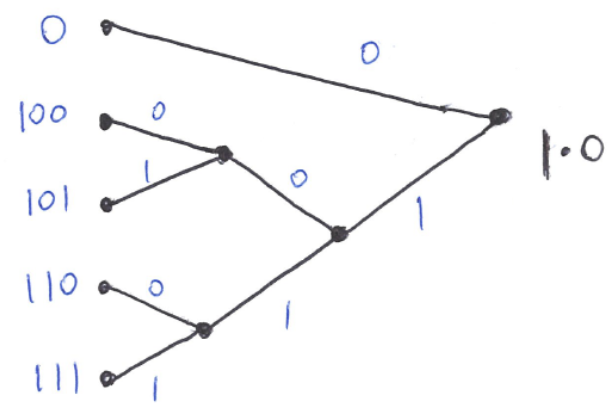
\includegraphics[width=\linewidth]{cd3236-huffman-code-tree.png} 
  \end{minipage}

  \begin{itemize}
    \item extension: using blocks of $n$ letters; Huffman coding with $\mathcal{X}^n$ 
      \\* $nH(X) \leq L(C) < nH(X) + 1$
      \\* $\quad \Rightarrow H(X) \leq$ avg. length per symbol $\leq H(X) + \frac{1}{n}$
      \begin{itemize}
        \item $\checkmark$ exploits \textit{memory}, better guarantee (even independent)
        \item $\times$ but it's harder to accurately know $P_{X_1 \dots X_n}$
        \item $\times$  alphabet size increases to $\vert \mathcal{X} \vert^n$ $\Rightarrow$ expensive to sort
      \end{itemize}
  \end{itemize}


  \section{03. BLOCK-WISE SOURCE CODING}

  \begin{itemize}
    \item \textbf{discrete memoryless source} 
      \begin{itemize}
        \item i.i.d. sequence $\mathbf{X} = (X_1, \dots, X_n)$
        \item $\mathbf{X}$ has \ildefinition{pmf} $P_{\mathbf{X}}(\mathbf{x}) = \Pi^n_{i=1} P_X(x_i)$ $\quad$(\textit{memoryless})
      \end{itemize}
    \item length-$n$ block $\mathbf{X}$
      $\Rightarrow$ integer $m \in \{1, \dots, M\}$
      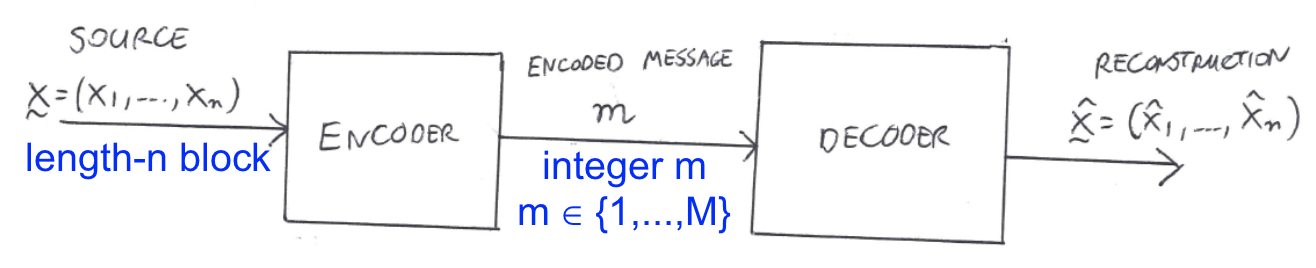
\includegraphics[width=0.9\linewidth]{cs3236-blockwise-source-coding.png} 
    \item \definition{error} 
      $P_e = \mathbb{P}[\hat{\mathbf{X}} \neq {\mathbf{X}}] = \sum_{\mathbf{x}: \textsc{DEC(ENC($x$))} \neq x} P_{\mathbf{X}}(\mathbf{x})$
    \item \definition{rate} $R = \frac{1}{n}\log_2 M$ $\;$ (compressed length $k = \log_2M$)
      \begin{itemize}
        \item lower rate = more compression ($M = 2^{nR}$)
        \item $R \leq H(X) + \epsilon$
      \end{itemize}
  \end{itemize}

  \begin{itemize}
    \item \definition{fixed length source coding theorem} $n, R, P_e$ tradeoff
      \begin{itemize}
        \item (\textbf{achievability}) if $R>H(X)$, then for any $\epsilon > 0$, we can get $P_e \leq \epsilon$ for large enough $n$ 
        \item (\textbf{converse}) if $R<H(X)$, then $\exists\epsilon > 0$ s.t. $\forall n, P_e > \epsilon$
      \end{itemize}
  \end{itemize}

  \subsection{Typical Sequences}

  \begin{tightcenter}
    \ildefinition{typical set}, \( {\displaystyle{ \mathcal{T}_n(\epsilon) = }} \) 
    \( {\displaystyle{ \left\{ \mathbf{x} \in \mathcal{X}^n : 2^{-n(H(X) + \epsilon)} \leq P_\mathbf{X}(\mathbf{x}) \leq 2^{-n(H(X)-\epsilon)} \right\} }} \) 
    where $\epsilon > 0$ is a (small) fixed constant
    \\* i.e. $P_{\mathbf{X}}({\mathbf{x}}) \simeq 2^{-nH({\mathbf{X}})}$
  \end{tightcenter}

  \begin{itemize}
    \item only assign a (unique) $m \in \{1, {\scriptscriptstyle\dots}, M-1\}$ if $\mathbf{x} \in \mathcal{T}_n(\epsilon)$
      \begin{itemize}
        \item choose ${\mathbf{x}}$ such that $\mathbb{P}[\mathbf{x} \in \mathcal{T}_n(\epsilon)] \simeq 1$
        \item map $\mathbf{x} \not\in \mathcal{T}_n(\epsilon)$ to dummy value $M$: $P_e = \mathbb{P}[\mathbf{X} \not \in \mathcal{T}_X]$
      \end{itemize}
  \end{itemize}

  \subsubsection{properties of a typical set}

  \begin{enumerate}
    \item (\textbf{equivalent definition}) $\mathbf{x} \in \mathcal{T}_n(\epsilon) \iff$  
      \( {\displaystyle{ H(X) - \epsilon \leq \frac{1}{n} \sum^n_{i=1} \log_2 \frac{1}{P_X(x_i)} \leq H(X) + \epsilon }} \) 
      \begin{itemize}
        \item $\mathbb{E}[\log P_X(x_i)] = H(X_i) = H(X)$
      \end{itemize}
    \item \( {\displaystyle{ \mathbb{P}[X \in \mathcal{T}_n(\epsilon)] \to 1 \;\; }} \)  as $n \to \infty \quad$ (\textbf{high probability})
    \item \( {\displaystyle{ \vert \mathcal{T}_n(\epsilon)\vert \leq 2^{n(H(X) + \epsilon)} \quad }} \)  (\textbf{cardinality upper bound})
    \item \( {\displaystyle{ \vert \mathcal{T}_n(\epsilon)\vert \geq (1-o(1)) 2^{n(H(X) - \epsilon)} \quad }} \)  
      \\*  where $o(1) \to 0$ as $n \to \infty$ (\textbf{cardinality lower bound})
  \end{enumerate}

  \begin{tightcenter}
    \ildefinition{asymptotic equipartition property}
    \\* as $n \to \infty$, the distribution is roughly uniform over $\mathcal{T}_n(\epsilon)$
  \end{tightcenter}

  \begin{itemize}
    \item with \textit{high probability} (2), a randomly drawn i.i.d. sequence $\mathbf{X}$ will be one of $\approx 2^{n(H(X))}$ sequences (3)(4),
      each of which has probability of $\approx 2^{-nH(X)}$ (definition of typical set)
  \end{itemize}

  \textbf{weak LoLN:} \( {\displaystyle{ \lim_{n \to \infty} \mathbb{P} \left[ \left\vert \frac{1}{n} \sum^n_{i=1} X_i - \mathbb{E}[X] \right\vert > \epsilon \right] = 0 }} \) 

  \textbf{LoLN:} $ \frac{1}{n}\sum^n_{i=1}X_i \to \mathbb{E}[X] $ as $n \to \infty$


  \subsection{Fano's Inequality}

  \begin{tightcenter}
    \ildefinition{Fano's Inequality}
    \setlength\abovedisplayskip{0pt}
    \setlength\belowdisplayskip{0pt}
    \setlength\abovedisplayshortskip{0pt}
    \setlength\belowdisplayshortskip{0pt}
    \begin{align*}
      H(X \vert \hat{X}) &\leq H_2(P_e) + P_e\log_2 (\vert\mathcal{X}\vert -1)  \\*
                         &\leq 1 + P_e \log_2 \vert \mathcal{X} \vert
    \end{align*}
  \end{tightcenter}

  \begin{itemize}
    \item intuition: if estimate $\hat{\mathbf{X}}$ is accurate (small $P_e$), then
      $I(\mathbf{X};\hat{\mathbf{X}}) \approx H(\mathbf{X}) = nH(X) \quad\quad \Rightarrow H(\mathbf{X}|\hat{\mathbf{X}}) \approx 0$
      \begin{itemize}
        \item $H_2(P_e)$ = uncertainty in "is $X=\hat{X}$"
        \item $\log_2(|\mathcal{X}|-1)$ = max uncertainty in the no case
      \end{itemize}
    \item proves \textit{converse} of \textbf{fixed length source coding theorem}
      $\quad\quad \Rightarrow \; P_e \geq \frac{1}{\log_2|\mathcal{X}|} (H(X) - R - \frac{1}{n})$
      % \begin{itemize}
      %   \item when $R<H(x)$, for scheme, $P_e \to 1$ as $n \to \infty$
      % \end{itemize}
  \end{itemize}


  \section{04. CHANNEL CODING}

  \begin{itemize}
    \item transmit $m \in \{1, \dots, M\} \quad$  ($M=2^k=2^{nR}$ for length-$k$)
    \item \ildefinition{codeword} $\mathbf{x}^{(m)} = (x_1^{(m)}, \dots, x_n^{(m)})$
      transmitted over the channel in $n$ uses; $\;$
      \ildefinition{codebook} $\mathcal{C} = \{\mathbf{x}^{(1)}, \dots, \mathbf{x}^{(M)}\}$
      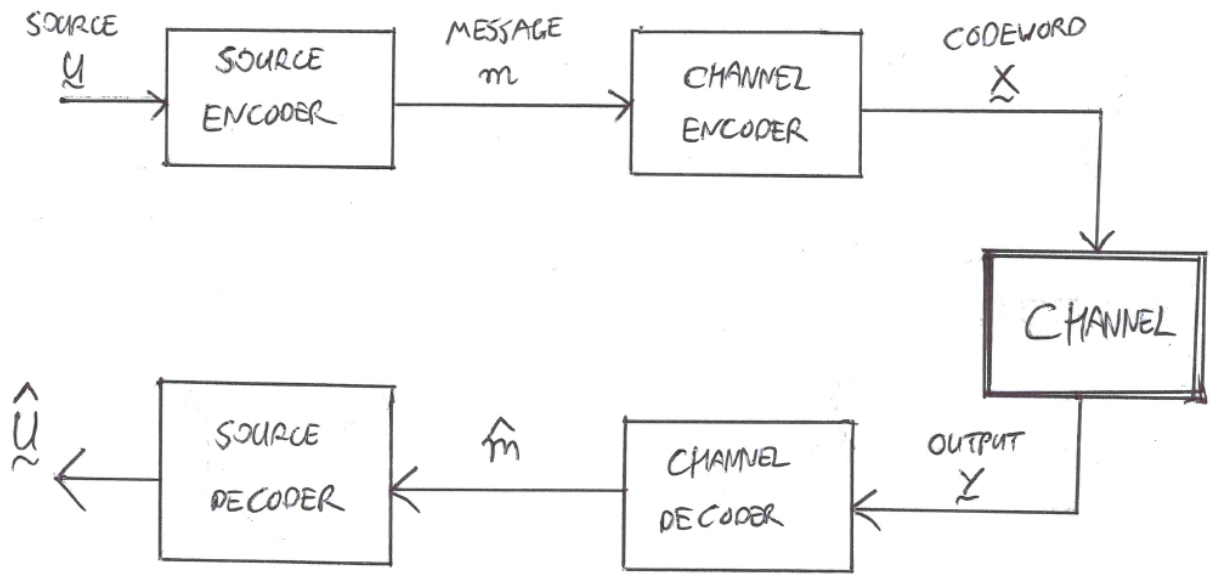
\includegraphics[width=0.9\linewidth]{cs3236-full-communication-setup.png} 
    \item \definition{memoryless} outputs are (conditionally) independent: $\mathbb{P}[Y=y \vert X=x] = \Pi^n_{i=1} P_{Y \vert X} (y_i \vert x_i)$
    \item \definition{error probability} $P_e = \mathbb{P}[\hat{m} \neq m]$
    \item \definition{rate} $R = \frac{1}{n} \log_2 M \quad\quad$ ($R \leq 1$ for binary channels)
      \begin{itemize}
        \item higher rate = sending faster (vs source coding: lower)
      \end{itemize}
    \item channel $P_{X|Y}$ is fixed; choose $P_X$ by codebook generation
  \end{itemize}

  \subsection{Channel Capacity}

  \begin{itemize}
    \item \definition[, $C$]{channel capacity} maximum of all rates $R$ such that, for any target error probability $\epsilon > 0$, $\exists$ block length $n$, codebook $\mathcal{C} = \{x^{(1)}, \dots, x^{(M)}\}$, such that $P_e \leq \epsilon$
  \end{itemize}

  \begin{tightcenter}
    \definition{channel coding theorem} $ \mathbb{P}_e \leq \epsilon \Leftrightarrow$ rate $<C$

    where the capacity
    \( {\displaystyle{ C=\max_{P_x} I(X;Y) }} \) 
  \end{tightcenter}

  \begin{itemize}
    \item (\textbf{achievability}) for any $R<C$, there exists a code of rate $\geq R$ with arbitrarily small $P_e$
    \item (\textbf{converse}) for any $R>C$, any code rate $\geq R$ cannot have arbitrarily small $P_e$ (for any codebook)
    \item noiseless/deterministic channel: $ C= \max_{P_X} H(X) = 1 $
    \item binary symmetric channel: $C = 1-H_2(\delta)$
    \item binary erasure channel ($\mathcal{Y} = \{0,1,e\}$, $\mathbb{P}[$erasure$]=\epsilon$):
      $ \quad C = \max_{P_X} (H(X) - \epsilon H(X)) = 1-\epsilon $
  \end{itemize}

  \subsection{Jointly Typical Sequences}

  \begin{tightcenter}
    a pair of $(\mathbf{x}, \mathbf{y})$ of length-$n$ input and output sequences is \ildefinition{jointly typical}  wrt a joint distribution $P_{XY}$ if 
    $2^{-n(H(X)+\epsilon)} \leq P_\mathbf{X}(\mathbf{x}) \leq 2^{-n(H(X)-\epsilon)}$
    $2^{-n(H(Y)+\epsilon)} \leq P_\mathbf{Y}(\mathbf{y}) \leq 2^{-n(H(Y)-\epsilon)}$
    $2^{-n(H(X,Y)+\epsilon)} \leq P_{\mathbf{XY}}(\mathbf{x}, \mathbf{y}) \leq 2^{-n(H(X,Y)-\epsilon)}$
  \end{tightcenter}

  \begin{itemize}
    \item aka: the $X$ seq, $Y$ seq, and joint $(X,Y)$ seq are all typical
    \item \definition[, $\mathcal{T}_n(\epsilon)$]{jointly typical set} set of all jointly typical seqs
  \end{itemize}

  \subsubsection{properties}

  \begin{enumerate}
    \item (\textbf{equivalent definition}) $\quad(\mathbf{x}, \mathbf{y}) \in \mathcal{T}_n(\epsilon) \iff $
      $\quad H(X) - \epsilon \leq \frac{1}{n} \sum^n_{i=1} \log_2 \frac{1}{P_X(x_i)} \leq H(X) + \epsilon$
      $\quad H(Y) - \epsilon \leq \frac{1}{n} \sum^n_{i=1} \log_2 \frac{1}{P_Y(y_i)} \leq H(Y) + \epsilon$
      $H(X, Y) - \epsilon \leq \frac{1}{n} {\displaystyle{\sum^n_{i=1}}} \log_2 \frac{1}{P_Y(x_i, y_i)} \leq H(X, Y) + \epsilon$

    \item (\textbf{high probability})
      $\mathbb{P}[(\mathbf{X}, \mathbf{Y}) \in \mathcal{T}_n(\epsilon)] \to 1$ as $n \to \infty$
    \item (\textbf{cardinality upper bound})
      \( {\displaystyle{ \vert \mathcal{T}_n(\epsilon) \vert \leq 2^{n(H(X,Y)+\epsilon)} }} \) 
    \item (\textbf{probability for independent sequences}) \\*
      if $(\mathbf{X}', \mathbf{Y}') \sim P_X(\mathbf{x}')P_Y(\mathbf{y}')$ are independent copies of  $(\mathbf{X}, \mathbf{Y})$, then the probability of joint typicality is 
      $\mathbb{P}[(\mathbf{X}', \mathbf{Y}') \in \mathcal{T}_n(\epsilon)] \leq 2^{-n(I(X;Y)-3\epsilon)}$
      \begin{itemize}
        \item X and Y drawn independently (instead of joint distribution) $\Rightarrow$ much lower probability of being typical
      \end{itemize}
  \end{enumerate}

  \subsubsection{Achievability via Random Coding}

  \begin{itemize}
    \item for a random $\mathcal{C}$, show $\mathbb{E}[P_e(\mathcal{C})] \leq \epsilon$ 
      (thus $\exists \mathcal{C}$ with $P_e \leq \epsilon$)
      \begin{itemize}
        \item if $!\exists m'$ s.t. $(\mathbf{X}^{(m')}, \mathbf{Y}) \in \mathcal{T}_n(\epsilon)$, set $\hat{m} = m'$
      \end{itemize}
      \item \( {\displaystyle{ P_e \leq \delta_n + M \times 2^{-n(I(X;Y) - 3\epsilon)}  }} \) 
      \item arbitrarily small $P_e$ for any $R$ close to $I(X;Y)$ (close to $C$)
  \end{itemize}

  \subsubsection{Converse via Fano's Inequality}

  \begin{itemize}
    \item note that $m \rightarrow \mathbf{X} \rightarrow \mathbf{Y} \rightarrow \hat{m}$ forms a \textbf{Markov chain}
  \end{itemize}

  $I(m; \hat{m}) \leq I(\mathbf{X};\mathbf{Y}) \leq nC$
  $\quad$ \( {\displaystyle{ \Rightarrow P_e \geq 1 - \frac{nC+1}{nR} }} \) 

  \section{05. CONTINUOUS-ALPHABET CH}

  \subsection{Differential Entropy}

  \begin{tightcenter}
    \ildefinition{differential entropy} of a continuous r.v. $X$ with pdf $f_X$ 
    \( {\displaystyle{ h(X) = \mathbb{E}_{f_X} \left[ \log_2 \frac{1}{f_X(X)} \right] }} \) 
    \\* \( {\displaystyle{ = \int_{\mathbb{R}} f_X(x) \log_2 \frac{1}{f_X(x)} \dx }} \) 

    \ildefinition{joint version},  \( {\displaystyle{ h(X,Y) = \mathbb{E} \left[ \log_2 \frac{1}{f_{XY} (x, y)} \right] }} \) 

    \ildefinition{conditional version},  \( {\displaystyle{ h(Y \vert X) = \mathbb{E}_{(X, Y)\sim f_{XY}} \left[ \log_2 \frac{1}{f_{Y \vert X} (Y \vert X)} \right] }} \) 
    \\* \( {\displaystyle{ = \int_{\mathbb{R}} f_X(x) h(Y \vert X=x) \dx }} \) 
    \\* where $(X,Y)$ have a joint density function $f_{XY}(x,y) = f_X(x)f_{Y|X}(y|x)$
  \end{tightcenter}

  \subsubsection{properties that still hold}

  \begin{itemize}
    \item (\textbf{chain rule}) $h(X_1, \dots, X_n) = \sum^n_{i=1} h(X_i \vert X_1, \dots, X_{i-1})$
    \item (\textbf{conditioning reduces entropy}) $\quad h(X \vert Y) \leq h(X)$
    \item (\textbf{sub-additivity}) $\quad h(X_1, \dots, X_n) \leq \sum^n_{i=1} h(X_i)$
    \item $h(X) = h(X+c)$ for some constant $c$
  \end{itemize}

  \textbf{properties of entropy that \textit{do not} hold}

  \begin{itemize}
    \item non-negativity: we can have $h(X) < 0$
    \item invariance under 1-1 transformations: $h(X) \neq h(\psi(X))$
    \item \textit{counterexample:} $Y=cX$.
      $\quad$ then $f_Y(y) = \frac{1}{\vert c \vert} f_X (\frac{y}{c})$, 
      \begin{itemize}
        \item which gives $h(Y) = \mathbb{E}[\log_2 \frac{1}{f_Y(y)}]$
          $= \mathbb{E}[\log_2 \frac{|c|}{f_X(Y/c)}] = \log_2|c| + h(X)$ $\quad \neq h(\psi(X))$
        \item violation of non-negativity: $\log_2|c| \to \infty$ as $c \to 0$
      \end{itemize}
  \end{itemize}

  \textbf{examples}

  \begin{itemize}
    \item $\textbf{Uniform}(a, b) \Rightarrow h(X) = \mathbb{E}[{\scriptscriptstyle \log_2 \frac{1}{f_X(x)}}] = \log_2(b-a)$
    \item \textbf{gaussian} $X \sim N(\mu, \sigma^2)$ $\Rightarrow$ $h(X) = \frac{1}{2}\log_2 (2\pi e \sigma^2)$
  \end{itemize}

  \subsection{Mutual information \& KL Divergence}

  \begin{tightcenter}
    \ildefinition{mutual information}
    \begin{align*}
      I(X;Y) &= h(Y) - h(Y \vert X) \\
             &= h(X) - h(X \vert Y) \\
             &= D(f_{XY} || f_X \times f_Y) \\
             &= \mathbb{E}_{f_{XY}} \left[ \log_2 \frac{f_{XY} (x,y)}{f_X(x) f_Y(y)} \right]
    \end{align*}
    \ildefinition{KL divergence}, 
    \( {\displaystyle{ D(f||g) = \int_{\mathbb{R}} f(x) \log_2 \frac{f(x)}{g(x)}\dx }} \) 
  \end{tightcenter}

  \textbf{properties: all hold}

  \begin{itemize}
    \item $I(X;Y) = I(\psi(X);\phi(Y))$ for invertible $\psi(\cdot)$ and $\phi(\cdot)$
  \end{itemize}

  \subsection{Gaussian Random Variables}

  if $X \sim N(\mu, \sigma^2)$, then $ h(X) = \frac{1}{2}\log_2 (2\pi e\sigma^2) $ 
  \begin{tightcenter}
    \ildefinition{maximum entropy property}\\*
    \( {\displaystyle{ h(X) \leq \frac{1}{2}\log_2 (2\pi e Var[X]) }} \) 
    \\* with equality $\iff X$ is Gaussian
  \end{tightcenter}

  \begin{itemize}
    \item for a given \textit{variance:} gaussian r.v. has highest entropy $h(\cdot)$ 
    \item for given \textit{values} ($X \in [a,b]$): uniform maximises $h(\cdot)$
  \end{itemize}

  \subsection{Gaussian Channel}

  a continuous channel is described by conditional pdf $f_{Y \vert X}$

  \begin{minipage}[c]{0.7\linewidth}{\color{black}{
        \begin{itemize}
          \item \definition{additive noise channels} $Y = X + Z$
            \begin{itemize}
              \item $Z$ is a noise term independent of $X$
              \item $f_{Y \vert X} (y \vert x) = f_Z(y-x)$
            \end{itemize}
        \end{itemize}
    }}
  \end{minipage}
  \begin{minipage}[c]{0.27\linewidth}
    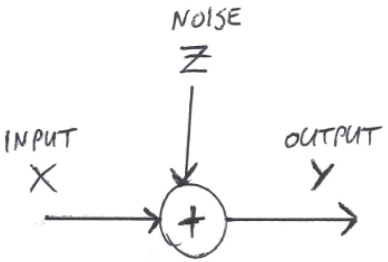
\includegraphics[width=0.95\linewidth]{cs3236-additive-noise-channel.png} 
  \end{minipage}

  \begin{itemize}
    \item \definition{additive white Gaussian noise (AWGN) channel} $Z \sim N(0, \sigma^2)$ for some noise variance $\sigma^2 > 0$
    \item \textbf{power constraint:} $\mathbb{E}[X^2] \leq P$
  \end{itemize}

  \subsubsection{Channel Capacity}

  \begin{itemize}
    \item channel capacity $C(P)$ is same as DMC, but codebooks are constrained to satisfy average power constraint
    \item for AWGN, capacity-achieving $f_X$ is gaussian: $N(0,P)$
  \end{itemize}
  \begin{tightcenter}
    \definition{AWGN capacity} $C(P) = \frac{1}{2} \log_2 (1 + \frac{P}{\sigma^2})$

    \definition{general} \( {\displaystyle{ C(P) = \max_{f_X : \mathbb{E}_{f_X} [X^2] \leq P} I(X;Y) }} \) 
  \end{tightcenter}

  \subsubsection{properties of Gaussian channel capacity}

  \begin{itemize}
    \item depends on $P, \sigma^2$ only through \textit{signal-to-noise ratio} $\frac{P}{\sigma^2}$
    \item $P=0 \Rightarrow SNR = 0 \Rightarrow$ $C=0$
    \item as $\sigma^2 \to 0$ for fixed $P$, then $SNR \to \infty, C \to \infty$
  \end{itemize}

  \begin{minipage}[c]{0.28\linewidth}
    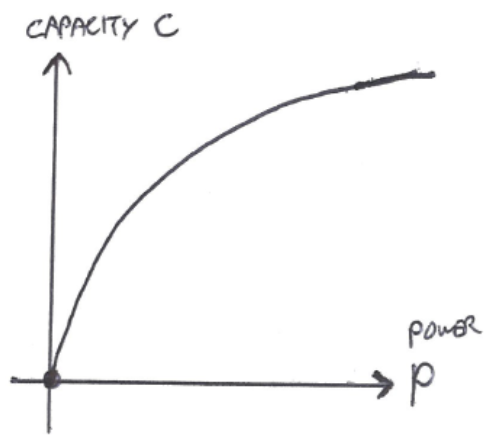
\includegraphics[width=\linewidth]{cs3236-capacity-to-snr.png} 
  \end{minipage}
  \begin{minipage}[c]{0.69\linewidth}\color{black}
      diminishing returns of increasing $P$
      \begin{itemize}
        \item small $\frac{P}{\sigma^2}$, $C(P) \approx \frac{P}{2\sigma^2}$ 
          \\* $\Rightarrow$ almost proportional to $P$
        \item large $\frac{P}{\sigma^2}$, $C(P) \approx \frac{1}{2}\log_2 \frac{P}{\sigma^2}$ 
          \\*  $\Rightarrow$ diminishing returns
      \end{itemize}
  \end{minipage}

  \section{06. PRACTICAL CHANNEL CODES}

  $\mathbf{u} {\scriptscriptstyle \in \{0, 1\}^k} = m {\scriptscriptstyle \in \{1,\dots,M\}} \Rightarrow \mathbf{x}^{(m)} \Rightarrow \mathbf{y}, P_e = \mathbb{P}[\hat{m} \neq m]$

  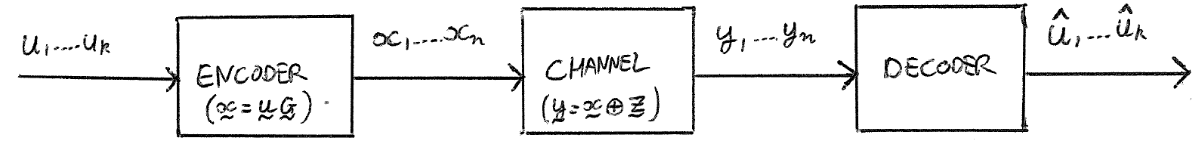
\includegraphics[width=\linewidth]{cs3236-linear-codes-diagram.png} 

  \begin{itemize}
    \item \definition{parity check} $c = b_1 \oplus \dots \oplus b_m$
      \begin{itemize}
        \item $\Rightarrow$ ensures an even number of 1's in the sequence
      \end{itemize}
  \end{itemize}

  \begin{itemize}
    \item channel: $\mathbf{y} = \mathbf{x} \oplus \mathbf{z}$; $\quad\mathbf{z} \in \{0, 1\}^n$ indicates flipped bits
    \item \ildefinition{rate} = $\frac{k}{n} = \frac{1}{n}\log_2 (\#\text{messages})$ since $M=2^k$ 
  \end{itemize}

  \subsubsection{Linear Codes}

  \begin{itemize}
    \item \definition{linear code} is comprised of parity checks
      \begin{itemize}
        \item $\oplus$ of any 2 codewords is another valid codeword
        \item if $\mathbf{u}, \mathbf{u}'$ correspond to codewords $\mathbf{x} = \mathbf{uG}, \mathbf{x}' = \mathbf{u}'\mathbf{G}$, then $\mathbf{x} \oplus \mathbf{x}'$ is also a codeword
      \end{itemize}
      \begin{tightcenter}
        \( {\displaystyle{ \mathbf{x} \oplus \mathbf{x}' = \mathbf{uG} \oplus \mathbf{u}'\mathbf{G} = (\mathbf{u} \oplus \mathbf{u}') \mathbf{G} }} \) 
      \end{tightcenter}
    \item \definition[parity-check code]{systematic} the first $k$ bits of $\mathbf{x}$ are always the original $k$ bits; remaining $n-k$ are parity checks
      $\quad x_i = \begin{cases} u_i &\text{if } i=1,\dots, k, \\ \bigoplus^k_{j=1} u_jg_{j,i} &\text{if } i = k+1,\dots, n \end{cases}$
    \item \definition[parity-check code]{general} all $n$ codeword bits may be arbitrary parity checks: $\bigoplus^k_{j=1} u_jg_{j,i}$ for  $i = 1, \dots, n$
  \end{itemize}

  \subsubsection{generator matrix}

  \begin{tightcenter}
    $\mathbf{x}$ is a codeword $\iff$ $\mathbf{x} = \mathbf{uG}$  (for some $\mathbf{u}$)
  \end{tightcenter}

  \begin{minipage}[c]{0.6\linewidth}\color{black}
    \begin{tightcenter}
      \ildefinition{generator matrix (general)}
      $\mathbf{G} = \begin{bmatrix}
        g_{1,1} & g_{1,2} & \cdots & g_{1,n} \\
        g_{2,1} & g_{2,2} & \cdots & g_{2,n} \\
        \vdots & \vdots & \ddots & \vdots \\
        g_{k,1} & g_{k,2} & \cdots & g_{k,n}
    \end{bmatrix} $
  \end{tightcenter}
  \end{minipage}
  \begin{minipage}[c]{0.37\linewidth}
    \begin{tightcenter}\color{black} 
      single-parity-check: 
      $ \mathbf{G}_{\text{parity}} = \left[\begin{smallmatrix}
          1 & 0 & 0 & 0 & 1 \\
          0 & 1 & 0 & 0 & 1 \\
          0 & 0 & 1 & 0 & 1 \\
          0 & 0 & 0 & 1 & 1 \\
      \end{smallmatrix}\right] $
      Hamming code:
      $ \mathbf{G} = \left[\begin{smallmatrix}
          1 & 0 & 0 & 0 & 1 & 1 & 0 \\
          0 & 1 & 0 & 0 & 1 & 0 & 1 \\
          0 & 0 & 1 & 0 & 0 & 1 & 1 \\
          0 & 0 & 0 & 1 & 1 & 1 & 1 \\
      \end{smallmatrix}\right] $
    \end{tightcenter}
  \end{minipage}

  \begin{itemize}
    \item \ildefinition{systematic}: leftmost $k\times k$ sub-matrix = identity matrix $I_k$
    \item codewords are linear combinations of the rows of $\mathbf{G}$
    \item $g_{j, i} = 1 \iff$ the $j$-th bit is used in the $i$-th parity check
  \end{itemize}

  \subsubsection{parity-check matrix}

  \begin{tightcenter}
    $\mathbf{xH} = \mathbf{0} \iff \mathbf{x}$ is a valid codeword \\*
    $\mathbf{G} = [\; \mathbf{I}_k \;\; \mathbf{P}\;]$ $\;\Longrightarrow\;$ $\mathbf{H} = \begin{bmatrix}
      \mathbf{P} \\ \mathbf{I}_{n-k}
    \end{bmatrix}$ \\*
  \end{tightcenter}

  \begin{minipage}[c]{0.6\linewidth}
    \begin{tightcenter}\color{black}
      \ildefinition{parity-check matrix (systematic)} \\*
      an $n \times (n-k)$ matrix
    \( {\displaystyle{ 
        \mathbf{H} = \left[\begin{smallmatrix}
          g_{1,k+1} & g_{1,k+2} & \cdots & g_{1,n} \\
          g_{2,k+1} & g_{2,k+2} & \cdots & g_{2,n} \\
          \vphantom{\int\limits^x}\smash{\vdots} & \smash{\vdots} & \smash{\ddots} & \smash{\vdots} \\
          g_{k,k+1} & g_{k,k+2} & \cdots & g_{k,n} \\
          1 & 0 & \cdots & 0 \\
          0 & 1 & \cdots & 0 \\
          \vphantom{\int\limits^x}\smash{\vdots} & \smash{\vdots} & \smash{\ddots} & \smash{\vdots} \\
          0 & 0 & \cdots & 1
        \end{smallmatrix}\right]
    }} \) 
  \end{tightcenter}
  \end{minipage}
  \begin{minipage}[c]{0.37\linewidth}
    \begin{tightcenter}\color{black}
      single-parity-check:
      $ \mathbf{H}_{\text{parity}} = \left[\begin{smallmatrix}
      1 \\ 1 \\ 1 \\ 1 \\ 1 \\ \end{smallmatrix}\right] $
      Hamming code:
      $ \mathbf{H}_{\text{Hamming}} = \left[\begin{smallmatrix}
          1 & 1 & 0 \\
          1 & 0 & 1 \\
          0 & 1 & 1 \\
          1 & 1 & 1 \\
          1 & 0 & 0 \\
          0 & 1 & 0 \\
          0 & 0 & 1 
      \end{smallmatrix}\right] $
    \end{tightcenter}
  \end{minipage}


  \begin{itemize}
    \item for $\mathbf{y=x\oplus z}$  ($\mathbf{z}$ is noise),
      \\* $\mathbf{yH} = (\mathbf{x}\oplus\mathbf{z})\mathbf{H} = \mathbf{(xH) \oplus (zH)} = \mathbf{zH}$
    \item $\left( \bigoplus^k_{j=1} x_j g_{j,i} \right) \oplus x_i = 0 $ since
      $\scriptscriptstyle x_i =  \bigoplus^k_{j=1} x_j g_{j,i}\text{ for } i\geq k+1$
  \end{itemize}


  \subsection{Distance Properties}

  \begin{itemize}
    \item \definition{Hamming distance} number of differing positions
      \begin{itemize}
        \item $d_H(\mathbf{x}, \mathbf{x}') = \sum^n_{i=1} \mathds{1}\{x_i \neq x_i'\}$
      \end{itemize}
    \item \definition{minimum distance} 
      \( {\displaystyle{ d_{\min} = \min_{\mathbf{x} \in \mathcal{C}, \mathbf{x}' \in \mathcal{C}: \mathbf{x} \neq \mathbf{x}'} d_H (\mathbf{x}, \mathbf{x'}) }} \) 
      \begin{itemize}
        \item correct $\leq d_{\min} - 1$ erasures and $\leq \frac{d_{\min}-1}{2}$ bit flips
      \end{itemize}
    \item \definition{weight} $w(\mathbf{x}) = \sum^n_{i=1} \mathds{1}\{w_i=1\} \quad$ (number of 1's)
      \begin{itemize}
        \item $w(\mathbf{x}) = \sum^n_{i=1} \mathds{1}\{w_i=1\}$
        \item for linear codes, min distance = min weight
          \begin{itemize}
            \item  \( {\displaystyle{ d_{\min} = \min_{\mathbf{x} \in \mathcal{C}: \mathbf{x} \neq 0} w(\mathbf{x}) }} \) 
              $\quad$ for $d_{\min} > 0$
          \end{itemize}
      \end{itemize}
  \end{itemize}

  \subsection{Minimum Distance Decoding}

  \subsubsection{maximum likelihood decoding}

  for any channel $P_{\mathbf{Y} \vert \mathbf{X}}$ and any codebook $\{ \mathbf{x}^{(1)}, \dots, \mathbf{x}^{(M)} \}$, 

  \begin{tightcenter}
    \definition{maximum-likelihood (ML) decoder} 
    minimises $P_e$
    \\* \( {\displaystyle{ \hat{m} = \argmax_{j = 1, \dots, M} P_{\mathbf{Y} \vert \mathbf{X}} (\mathbf{y} \vert \mathbf{x}^{(j)}) }} \) 
  \end{tightcenter}

  for BSC, ML decoding is equivalent to 
  \begin{tightcenter}
    \ildefinition{minimum (Hamming) distance decoding}
    \\* \( {\displaystyle{ \argmax_{j=1,\dots, M} P_{\mathbf{Y}\vert \mathbf{X}} (\mathbf{y} \vert \mathbf{x}^{(j)}) =  \argmin_{j=1,\dots, M} d_H (\mathbf{x}^{(j)}, \mathbf{y}) }} \) 
  \end{tightcenter}

  \subsubsection{syndrome decoding}

  for linear codes for the BSC, 

  \begin{itemize}
    \item \definition{syndrome} $\mathbf{S} = \mathbf{zH} = \mathbf{yH}$ 
      $\quad\quad\Rightarrow 1 \times (n-k)$ vector
    \item the \textit{minimum-distance codeword} to $\mathbf{y}$ is
      \begin{enumerate}
        \item \( {\displaystyle{ \hat{\mathbf{z}} = \argmin_{\mathbf{z'} : \mathbf{z'H=S}} w(\mathbf{z'}) }} \)  
          $\quad$ (i.e. $\mathbf{z}'$ with fewest 1's)
        \item $\hat{\mathbf{x}} = \mathbf{y} \oplus \hat{\mathbf{z}}$
      \end{enumerate}
    \item \textit{Proof.} define $\mathbf{z}^{(i)} = \mathbf{x}^{(i)}\oplus \mathbf{y}$ $\Rightarrow$ $d_H (\mathbf{x}^{(i)} \oplus \mathbf{y}) = w(\mathbf{z}^{(i)})$
  \end{itemize}

\end{multicols*}

\end{document}
